\section{An\'alisis de resultados}

\subsection{High-pass}

\ref{fig:ej2_HP_bode}

\begin{figure*}
	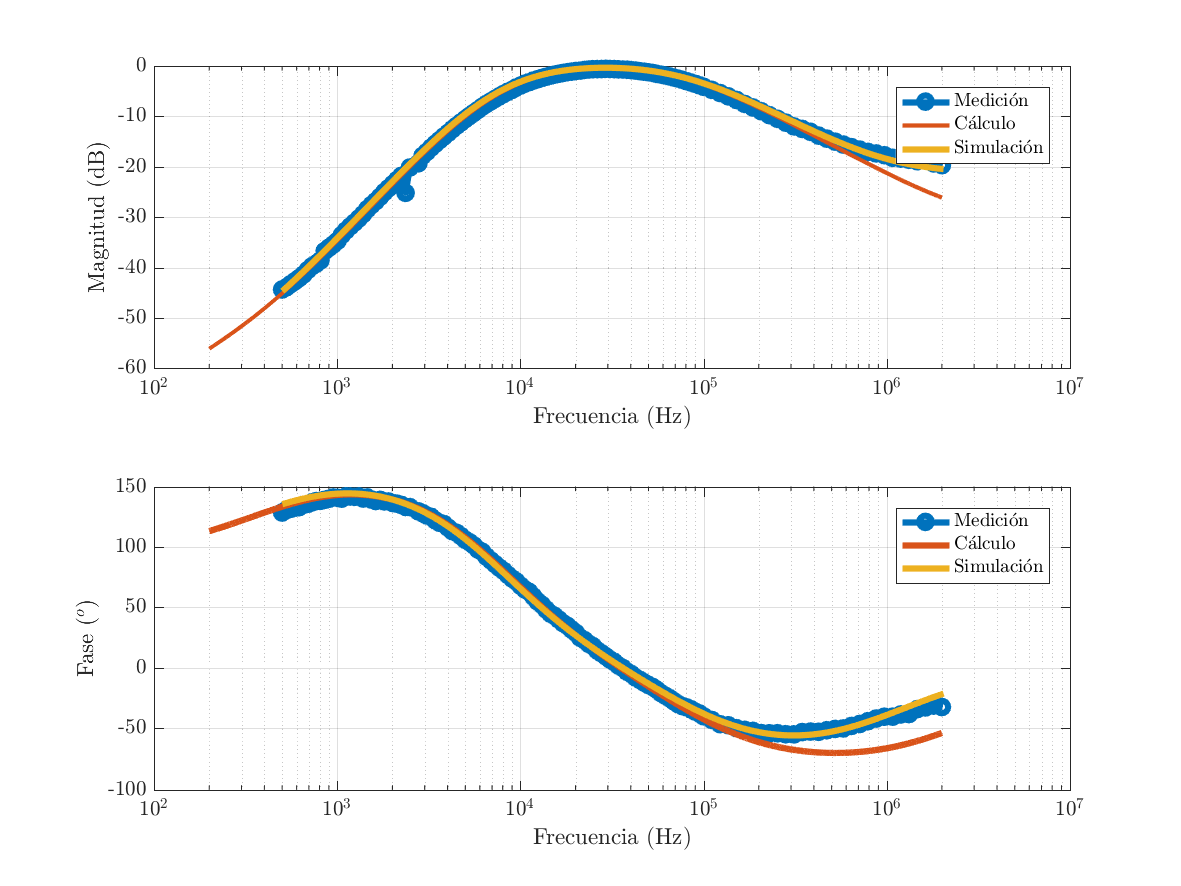
\includegraphics[width=\textwidth]{imagenes/HP_bode}
	\label{fig:ej2_HP_bode}
	\caption{Respuesta en frecuencia del filtro high-pass calculada, simulada, y medida}
\end{figure*}

\subsection{Low-pass}

\ref{fig:ej2_LP_bode}

\begin{figure*}
	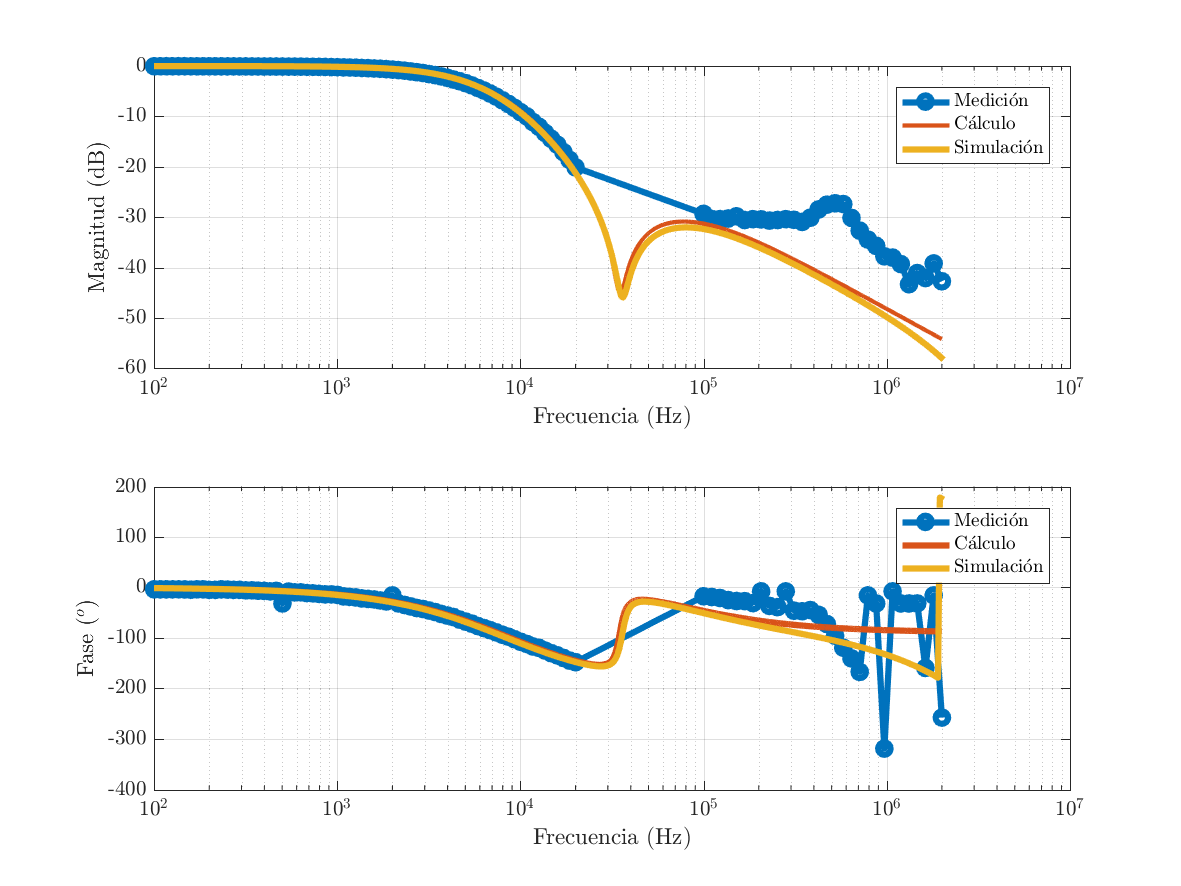
\includegraphics[width=\textwidth]{imagenes/LP_bode}
	\label{fig:ej2_LP_bode}
	\caption{Respuesta en frecuencia del filtro low-pass calculada, simulada, y medida. El caculo fue hecho para salida diferencial, y la simulacion y la medicion para la salida del restador}
\end{figure*}


\subsection{Band-pass}

\ref{fig:ej2_BP_bode}
\begin{figure*}
	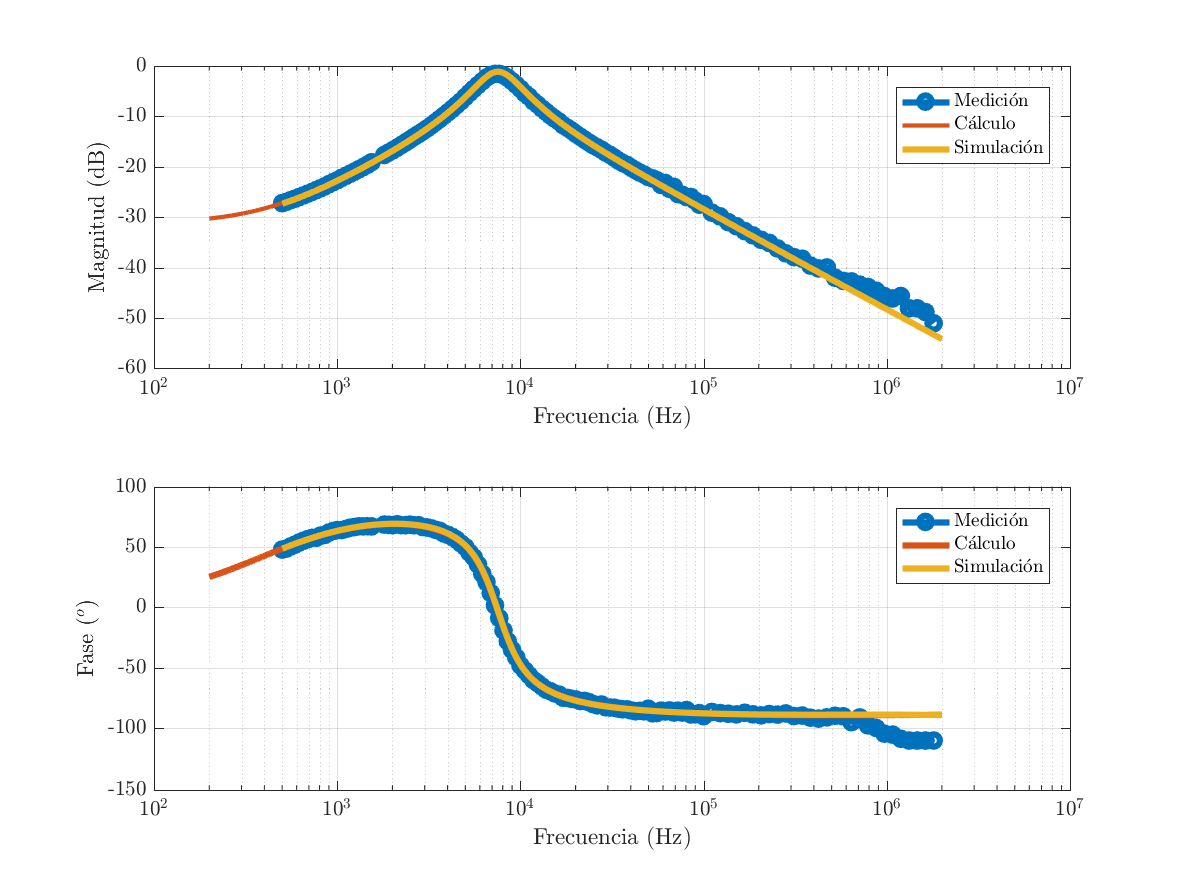
\includegraphics[width=\textwidth]{imagenes/BP_bode}
	\label{fig:ej2_BP_bode}
	\caption{Respuesta en frecuencia del filtro band-pass calculada, simulada, y medida}
\end{figure*}


\subsection{Band-reject}

\ref{fig:ej2_BR_bode}
\begin{figure*}
	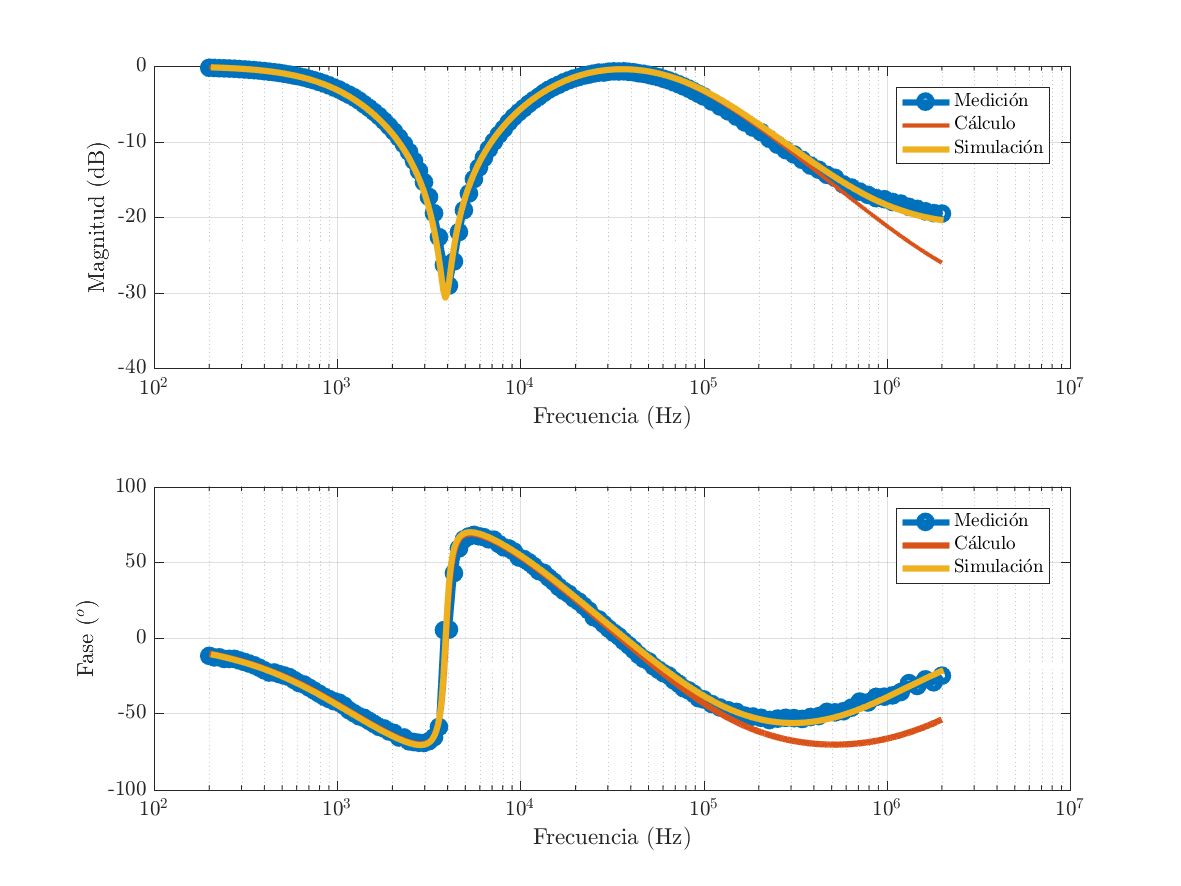
\includegraphics[width=\textwidth]{imagenes/BR_bode}
	\label{fig:ej2_BR_bode}
	\caption{Respuesta en frecuencia del filtro band-reject calculada, simulada, y medida}
\end{figure*}

